\documentclass[a4paper,12pt]{article}
\usepackage{mypreamble}

%% Page setup
\geometry{
    margin=2cm,
    includehead,
    % includefoot,
    headsep=\baselineskip,
}
\pagestyle{fancy}
\fancyfoot{}
\MakeDoubleHeader% {<l1>}{<l2>}{<r1>}{<r2>}
    {\TextHomeworkEng~\#3}
    {Boolean Algebra}
    {\TextDiscreteMathEng}
    {\IconFall~Fall 2023}

%% Add custom setup below

\usepackage{circuitikz}

\ctikzset{
    logic ports=ieee,
    logic ports/scale=0.7,
}

\newenvironment{smallcases}{%
    \bigl\lbrace\begin{smallmatrix}%
}{%
    \end{smallmatrix}%
}


\begin{document}
\selectlanguage{english}

\begin{tasks}
    %% Task: Karnaugh maps.
    \item Perform the following steps:
    \begin{subtasks}
        \item Calculate the SHA-256 hash~$h$ of the string $s = \text{\enquote{DM Fall 2023 HW3}}$ (without quotes, with all spaces, encoded in UTF-8).
        Convert hash~$h$ to a 256-bit binary string~$b$ (prepend leading zeros if necessary).
        Cut the binary string~$b$ into eight 32-bit slices $r_1, \dotsc, r_8$, \eg $r_2 = b_{33 \dd 64}$.
        Xor all slices into a 32-bit string $d = r_1 \xor \dotsb \xor r_8$.
        Compute $w = d \xor \mathtt{0x24d03294}$.

        \item Draw the Karnaugh map (use a template below) for a function $f(A,B,C,D,E)$ defined by the truth table~$w = (w_{1} \dots w_{32})$ (MSB corresponds to~$f(\vvmathbb{0}) = w_{1}$, LSB to~$f(\vvmathbb{1}) = w_{32}$).

        \item Use K-map to find the minimal DNF and minimal CNF for th function $f$.

        \item Use K-map to find the number of prime implicants, \ie the size of BCF\@.
        % \footnote{Here, consider only implicants represented as product terms.}

        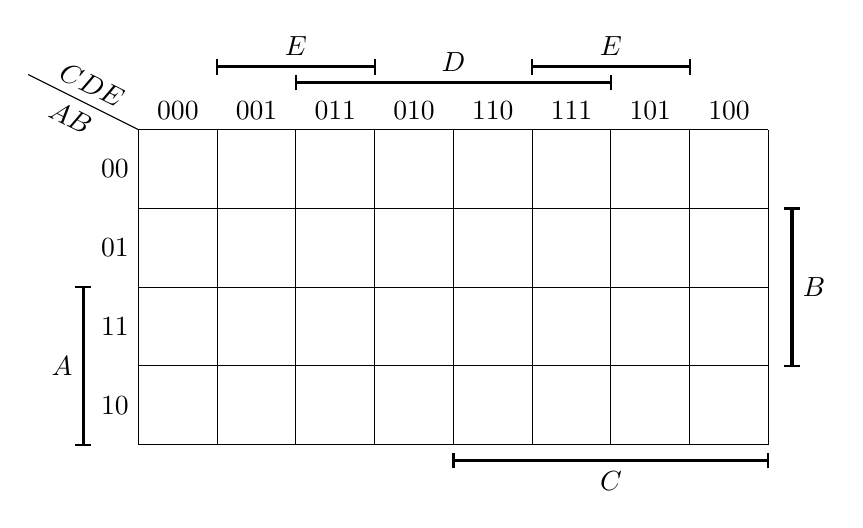
\begin{tikzpicture}[]
            \def\sidelinepaw{0.1}
            \newcommand\sidelineV[4]{% {<start>}{<height>}{<node-style>}{<node-text>}
                \coordinate (start) at #1;
                \draw[thick] (start) +(-\sidelinepaw,0) -- +(\sidelinepaw,0);
                \draw[thick] (start)++(0,#2) +(-\sidelinepaw,0) -- +(\sidelinepaw,0);
                \draw[very thick] (start) -- node[#3]{#4} ++(0,#2);
            }
            \newcommand\sidelineH[4]{% {<start>}{<width>}{<node-style>}{<node-text>}
                \coordinate (start) at #1;
                \draw[thick] (start) +(0,-\sidelinepaw) -- +(0,\sidelinepaw);
                \draw[thick] (start)++(#2,0) +(0,-\sidelinepaw) -- +(0,\sidelinepaw);
                \draw[very thick] (start) -- node[#3]{#4} ++(#2,0);
            }

            \draw (0,0) grid (8,4);
            \node[above] at (0.5,4) {000};
            \node[above] at (1.5,4) {001};
            \node[above] at (2.5,4) {011};
            \node[above] at (3.5,4) {010};
            \node[above] at (4.5,4) {110};
            \node[above] at (5.5,4) {111};
            \node[above] at (6.5,4) {101};
            \node[above] at (7.5,4) {100};
            \node[left] at (0,0.5) {10};
            \node[left] at (0,1.5) {11};
            \node[left] at (0,2.5) {01};
            \node[left] at (0,3.5) {00};
            \draw (0,4) -- node[sloped,below]{$AB$~~} node[sloped,above]{$CDE$} ++(-1.4,.7);

            \sidelineV{(-0.7,0)}{2cm}{left}{$A$}
            \sidelineV{(8.3,1)}{2}{right}{$B$}
            \sidelineH{(4,-0.2)}{4}{below}{$C$}
            \sidelineH{(2,4.6)}{4}{above}{$D$}
            \sidelineH{(1,4.8)}{2}{above}{$E$}
            \sidelineH{(5,4.8)}{2}{above}{$E$}
        \end{tikzpicture}
    \end{subtasks}


    %% Task: Find minimal DNF,CNF,etc using Karnaugh map, and find Zhegalkin polynomial.
    \item For each given function $f_i$ of 4 arguments, draw the Karnaugh map and use it to find BCF, minimal DNF, and minimal CNF\@.
    Additionally, construct ANF (Zhegalkin polynomial) using either the K-map, the tabular (\enquote{triangle}) method or the Pascal method --- use each method at least once.

    \makeatletter
    \newtcolorbox{notebox}[1][]{%
        enhanced jigsaw, % better frame drawing
        borderline west={1pt}{0pt}{black}, % straigh vertical line at the left edge
        sharp corners, % no rounded corners
        boxrule=0pt, % no real frame,
        % fonttitle={\large\bfseries},
        fonttitle={\bfseries},
        coltitle={black},  % Black colour for title
        title={Note},  % Fixed title
        attach title to upper, % Move the title into the box
        after title={:\ },
        colback=gray!10,
        % right=0pt,
        top=0pt,
        bottom=0pt,
        frame hidden,
        baseline={\tcb@height-2\kvtcb@boxsep+\baselineskip-2\lineskip},
        #1
    }
    \makeatother

    \begin{notebox}
        \RaggedRight
        WolframAlpha\Href{https://www.wolframalpha.com} interprets the query \enquote{$n$-th Boolean function of $k$ variables} in a reverse manner.
        In order to employ WolframAlpha properly, manually flip the truth table beforehand, \eg the correct query for $f^{(2)}_{10}$ is \enquote{5th~Boolean function of 2~variables}\Href{https://www.wolframalpha.com/input?i=5th+boolean+function+of+2+variables}, which gives $f^{(2)}_{10} = \neg x_2$, since $\mathtt{rev}(1010_2) = 0101_2 = 5_{10}$.
    \end{notebox}

    \begin{multicols}{2}
    \begin{subtasks}
        \item $f_{\arabic{subtasksi}} = f^{(4)}_{47541}$
        \item $f_{\arabic{subtasksi}} = \sum m (1,4,5,6,8,12,13)$
        \item $f_{\arabic{subtasksi}} = f^{(4)}_{51011} \xor f^{(4)}_{40389}$
        \item $f_{\arabic{subtasksi}} = A\overline{B}D + \overline{A}\,\overline{C}D + \overline{B}C \overline{D} + A\overline{C}D$
    \end{subtasks}
    \end{multicols}


    %% Task: Convert to CNF.
    \item Convert the following formulae to CNF.

    \begin{multicols}{2}
    \begin{subtasks}
        \item $X \iff (A \land B)$
        \item $Z \iff \biglor\nolimits_{i} C_i$
        \item $D_1 \xor \dotsb \xor D_n$
        \item $\operatorname{majority}(X_1, X_2, X_3)$ \footnote{Majority function\Href{https://en.wikipedia.org/wiki/Majority_function} is a Boolean function that is 1 iff the majority (more than half) of the inputs are 1.}
        \item $R \implies (S \implies (T \implies \bigland\nolimits_{i} F_i))$
        \item $M \implies (H \iff \biglor\nolimits_{i} D_i)$
    \end{subtasks}
    \end{multicols}


    % Task: Truth table for a circuit.
    \item Compute the truth table for the function $f \colon \Bool^3 \to \Bool^2$ (with the semantics $\Triple{A,B,C} \mapsto \Pair{f_{(1)}, f_{(2)}}$) represented with the following circuit.

    % \vspace{4pt}
    % f_(6,210)
    \begin{circuitikz}[]
        \node (A) at (0,3) {$A$};
        \node (B) at (0,1) {$B$};
        \node (C) at (0,0) {$C$};
        \draw
            (A.east) +(.7,0) coordinate(jA)
            (B.east) +(.7,0) coordinate(jB)
            (C.east) +(2,0) coordinate(jC)

            % g6 = AND(A, g5)
            (A.east) to[short,o-] ++(10,0) node[and port,anchor=in 1](g6){}
            % g3 = NOR(g2, C)
            (C.east) to[short,o-] ++(4,0) node[nor port,anchor=in 2](g3){}
            % g2 = AND(A, B)
            ($(jA)!0.5!(jB)$) ++(1,0) node[and port](g2){}
            % joint after g2
            (g2.out) +(0.5,0) coordinate(jg2)
            % g4 = AND(g2, C)
            (g2.out) -- ++(1.5,0) node[and port,anchor=in 1](g4){}
            % g5 = NOR(g4, g3)
            (g4.out) -- ++(1,0) node[nor port,anchor=in 1](g5){}
            % g1 = OR(A, B)
            (B.east) to[short,o-] ++(10,0) node[or port,anchor=in 2](g1){}
            % g7 = NAND(B, g5)
            (g1) ++ (0,-1) node[nand port](g7){}
            % g8 = NAND(g1, g7)
            (g1.out) -- ++(1,0) node[nand port,anchor=in 1](g8){}

            % joint after g5
            (g5.out) +(0.5,0) coordinate (jg5)
            % joint before g6
            (g6.in 1) +(-0.5,0) coordinate (jg6)
            % joint before g1
            (g1.in 2) +(-0.5,0) coordinate (jg1)

            % outputs
            (g8.out) to[short,-o] ++(0.3,0) node[anchor=west](OUT2){$f_{(2)}$}
            (g6.out) to[short,-o] (g6.out -| OUT2.west) node[anchor=west](OUT1){$f_{(1)}$}

            % interconnections
            (jA) to[short,*-] (jA |- g2.in 1) -- (g2.in 1)
            (jB) to[short,*-] (jB |- g2.in 2) -- (g2.in 2)
            (jg2) to[short,*-] (jg2 |- g3.in 1) -- (g3.in 1)
            (jC) to[short,*-] +(0,0) to[out=90,in=180] (g4.in 2)
            (g3.out) to[out=0,in=180] (g5.in 2)
            (g5.out) to[short,-*] (jg5) to[out=0,in=180] (g6.in 2)
            (jg6) to[short,*-] +(0,0) |- (g1.in 1)
            (jg1) to[short,*-] +(0,0) |- (g7.in 1)
            (jg5) |- (g7.in 2)
            (g7.out) to[out=0,in=180] (g8.in 2)
        ;
    \end{circuitikz}
    \vspace{6pt}


% \tcbset{
%     dang/.style={
%         enhanced,
%         breakable,
%         fonttitle=\bfseries,
%         before skip=2mm,
%         after skip=2mm,
%         colframe=blue!40!black,
%         colback=white,
%         colbacktitle=blue!40!black,
%         boxrule=0.5mm,
%         arc is angular,
%         attach boxed title to top left={
%             xshift=1cm,
%             yshift*=1mm-\tcboxedtitleheight
%         },
%         varwidth boxed title*=-3cm,
%         boxed title style={
%             frame code={
%                 \path[fill=tcbcolback!30!black]
%                     ([yshift=-1mm,xshift=-1mm]frame.north west)
%                     arc[start angle=0,end angle=180,radius=1mm]
%                     ([yshift=-1mm,xshift=1mm]frame.north east)
%                     arc[start angle=180,end angle=0,radius=1mm];
%                 \path[left color=tcbcolback!60!black,
%                       right color=tcbcolback!60!black,
%                       middle color=tcbcolback!80!black]
%                     ([xshift=-2mm]frame.north west) -- ([xshift=2mm]frame.north east)
%                     [rounded corners=1mm]-- ([xshift=1mm,yshift=-1mm]frame.north east)
%                     -- (frame.south east) -- (frame.south west)
%                     -- ([xshift=-1mm,yshift=-1mm]frame.north west)
%                     [sharp corners]-- cycle;
%             },
%             interior engine=empty,
%         },
%     },
% }

% \newtcolorbox{defbox}[2][]{% [<style>]{<title>}
%     dang,
%     title={#2},
%     #1
% }

%     %% Task: Post's theorem.
%     \item Prove rigorously the following theorem.

%     \begin{defbox}{Post's Functional Completeness Theorem}
%         A system $F$ of boolean functions is functionally complete (\ie clone of the given set~$F$ is equal to the set of all Boolean functions~$\mathbb{F}$) for each of the five Post's classes ($T_0$,~$T_1$, $S$, $M$,~$L$), there is a function $f \in F$ which does not belong to that class.
%         % In other words, $F$~contains:
%         % \begin{itemize}[left=1pc]
%         %     \item at least one function that does \textit{not} preserve zero, \ie $\exists f \in F: f \notin T_0$, and
%         %     \item at least one function that does \textit{not} preserve one, \ie $\exists f \in F: f \notin T_1$, and
%         %     \item at least one function that is \textit{not} self-dual, \ie $\exists f \in F: f \notin S$, and
%         %     \item at least one function that is \textit{not} monotonic, \ie $\exists f \in F: f \notin M$, and
%         %     \item at least one function that is \textit{not} linear function, \ie $\exists f \in F: f \notin
%         %     L$.
%         % \end{itemize}

%         % \tcblower

%         % A function $f$ is \textbf{zero-preserving} iff it is \texttt{False} on the zero-valuation:\par
%         % \quad$f \in T_0 \iff f(\vvmathbb{0}) = 0$

%         % A function $f$ is \textbf{one-preserving} iff it is \texttt{True} on the one-valuation:\par
%         % \quad$f \in T_1 \iff f(\vvmathbb{1}) = 1$

%         % A function $f$ is \textbf{self-dual} iff it is dual to itself:\par
%         % \quad$f \in S \iff \forall x_1,\dotsc,x_n \in \Bool : f(x_1, \dotsc, x_n) = \overline{f}(\overline{x}_1, \dotsc, \overline{x}_n)$.

%         % A function $f$ is \textbf{monotonic} iff, for every increasing input, the function does not decrease:\par
%         % \quad$f \in M \iff \forall a,b \in \Bool^n: a \preceq b \implies f(a) \leq f(b)$.

%         % Comparison of inputs $a,b \in \Bool^n$ is defined as follows:\par
%         % \quad$\displaystyle a \preceq b \iff \biglandclap{1 \leq i \leq n} a_i \leq b_i$

%         % A function $f$ is \textbf{linear} iff its Zhegalkin polynomial is linear (\ie has a degree at most 1):\par
%         % \quad$f \in L \iff \operatorname{deg} f_{\xor} \leq 1$
%     \end{defbox}


    %% Task: Functional completeness.
    \item For each given system of functions $F_i$, determine whether it is functionally complete using Post's criterion.
    For each basis~$F_i$, use it to rewrite the function $g(A,B,C) = A \implies ((\neg A \xor B) \land \neg C)$.
    Draw a combinational Boolean circuit for each resulting formula.

    \begin{multicols}{2}
    \begin{subtasks}
        \item $F_{\arabic{subtasksi}} = \Set{ \land, \lor, \neg }$
        \item $F_{\arabic{subtasksi}} = \Set{ f^{(2)}_{14} }$
        \item $F_{\arabic{subtasksi}} = \Set{ \implies, \centernot\implies }$
        \item $F_{\arabic{subtasksi}} = \Set{ 1, \iff , \land }$
    \end{subtasks}
    \end{multicols}


    %% Task: Prove that Zhegalkin basis is complete.
    \item Show \--- without using Post's criterion \--- that the Zhegalkin basis $\Set{\xor, \land, 1}$ is functionally complete.
    % TODO: ... and irreducible.


    %% Task: Binary-to-Gray conversion.
    \item Construct a minimal (in terms of the number of gates) Boolean circuit that implements the conversion of 4-bit binary numbers to Gray code\Href{https://en.wikipedia.org/wiki/Gray_code}, \ie the function $f \colon \Bool^4 \to \Bool^4$ with the semantics $(b_3,b_2,b_1,b_0) \mapsto (g_3,g_2,g_1,g_0)$, \eg $\mathtt{0000}_{2} \mapsto \mathtt{0000}_{\mathrm{Gray}}$, and $\mathtt{1001}_{2} \mapsto \mathtt{1101}_{\mathrm{Gray}}$.
    Use only $\mathtt{NAND}$ and $\mathtt{NOR}$ logic gates.


    % Task: Comparator.
    \item Construct a circuit that compares the two-bit integers $(x_1 x_0)_2$ and $(y_1 y_0)_2$, returning an output of~1 when the first of these numbers is larger and an output of~0 otherwise.


    % Task: Multiplier.
    \item Construct a circuit that computes the product of the two-bit integers $(x_1 x_0)_2$ and $(y_1 y_0)_2$.
    The circuit should have four-bit output $(p_3 p_2 p_1 p_0)_2$.


    %% Task: MUX.
    \item Consider a Boolean function $\operatorname{ITE} \colon \Bool^3 \to \Bool$ defined as follows:
    $\operatorname{ITE}(c,x,y) = \begin{smallcases}
        x & \text{if } c = 0 \\
        y & \text{if } c = 1
    \end{smallcases}$.
    Construct a formula for it using the standard Boolean basis $\Set{\land, \lor, \neg}$.
    Determine whether the set $\Set{\operatorname{ITE}}$ is functionally complete.


    \makeatletter
    \newtcolorbox{defbox}[1][]{%
        enhanced jigsaw, % better frame drawing
        borderline west={1pt}{0pt}{black}, % straigh vertical line at the left edge
        sharp corners, % no rounded corners
        boxrule=0pt, % no real frame,
        fonttitle={\bfseries},
        coltitle={black},  % Black colour for title
        attach title to upper, % Move the title into the box
        after title={\ },
        colback=gray!10,
        % right=0pt,
        top=0pt,
        bottom=0pt,
        frame hidden,
        baseline={\tcb@height-2\kvtcb@boxsep+\baselineskip-2\lineskip},
        #1
    }
    \makeatother

    %% Task: BDD.
    \item For each given function~$f_i$, construct an Reduced Ordered Binary Decision Diagram (ROBDD) using the natural order $x_1 \prec x_2 \prec \dotsb \prec x_n$.
    Determine whether the ROBDD can be reduced by using a different variable order \--- if so, draw it.

    \begin{defbox}
        Binary Decision Diagram\Href{https://en.wikipedia.org/wiki/Binary_decision_diagram} (BDD) is a representation of a Boolean function as a directed acyclic graph, which consists of \emph{decision} nodes and two \emph{terminal} nodes (0~and~1).
        Each decision node is labeled by a Boolean variable~$x_i$ and has two child nodes called \emph{low} and \emph{high}.
        The edge from node to a low (high) child represents an assignment of the value \texttt{FALSE} (\texttt{TRUE}, respectively) to variable~$x_i$.
        A path from the root node to the 1-terminal (0-terminal) corresponds to an assignment for which the represented Boolean function is true (false, respectively).

        BDD is called \emph{ordered} if different variables appear in the same order on all paths from the root.
        For example, if the natural order $x_1 \prec x_2 \prec \dotsb \prec x_n$ is used, the root is marked with the variable~$x_1$, its children with~$x_2$, \textit{etc}.
        Note that some variables in the order can be skipped, if necessary.

        BDD is called \emph{reduced} if it does not contain a node $v$ with $\operatorname{high}(v) = \operatorname{low}(v)$, and there does not exist a pair of nodes $u,v$ such that the sub-OBDDs rooted in $u$ and $v$ are isomorphic.
    \end{defbox}

    \begin{multicols}{2}
    \begin{subtasks}
        \item $f_{\arabic{subtasksi}}(x_1,\dots,x_4) = x_1 \xor x_2 \xor x_3 \xor x_4$
        \item $f_{\arabic{subtasksi}}(x_1,\dots,x_5) = \operatorname{majority}(x_1,\dotsc,x_5)$
        \item $f_{\arabic{subtasksi}}(x_1,\dots,x_4) = \sum m(1,2,5,12,15)$
        \item $f_{\arabic{subtasksi}}(x_1,\dots,x_6) = x_1 x_4 + x_2 x_5 + x_3 x_6$
    \end{subtasks}
    \end{multicols}

    % \item \ldots
\end{tasks}

\end{document}
